\documentclass[11pt]{article}

\usepackage[margin=1in]{geometry}
\usepackage{amsfonts, amsmath, amssymb}
\usepackage[none]{hyphenat}
\usepackage{fancyhdr}
\usepackage{graphicx}
\usepackage{float}
\usepackage[nottoc, notlot, notlof]{tocbibind}
\usepackage{hyperref}
\usepackage[french]{babel}

\pagestyle{fancy}
\fancyhead{}
\fancyfoot{}
%\fancyhead[L]{\slshape \MakeUppercase{Radio}}
\fancyhead[R]{\slshape Projet Réseaux}
\fancyfoot[C]{\thepage}
\renewcommand{\footrulewidth}{0pt}

\parindent 0ex %
\renewcommand{\baselinestretch}{1.5}

\begin{document}

\begin{titlepage}
\begin{center}
\vspace*{1cm}
\Large{\textbf{Projet Réseaux}}\\
\vfill
\line(1,0){400}\\[1mm]
\huge{\textbf{Simulation d'un protocole de routage à vecteur de distances}}\\[3mm]
\Large{\textbf{- Rapport -}}\\[1mm]
\line(1,0){400}\\
\vfill
Abdelkrim ESSAFSYFY\\
Paul ONDAFE MATOCK\\
Année académique 2020-2021
\end{center}
\end{titlepage}

\tableofcontents
\thispagestyle{empty}
\clearpage
\setcounter{page}{1}

\section{Exercice 2.2}
\begin{figure} [h!]
\centering
  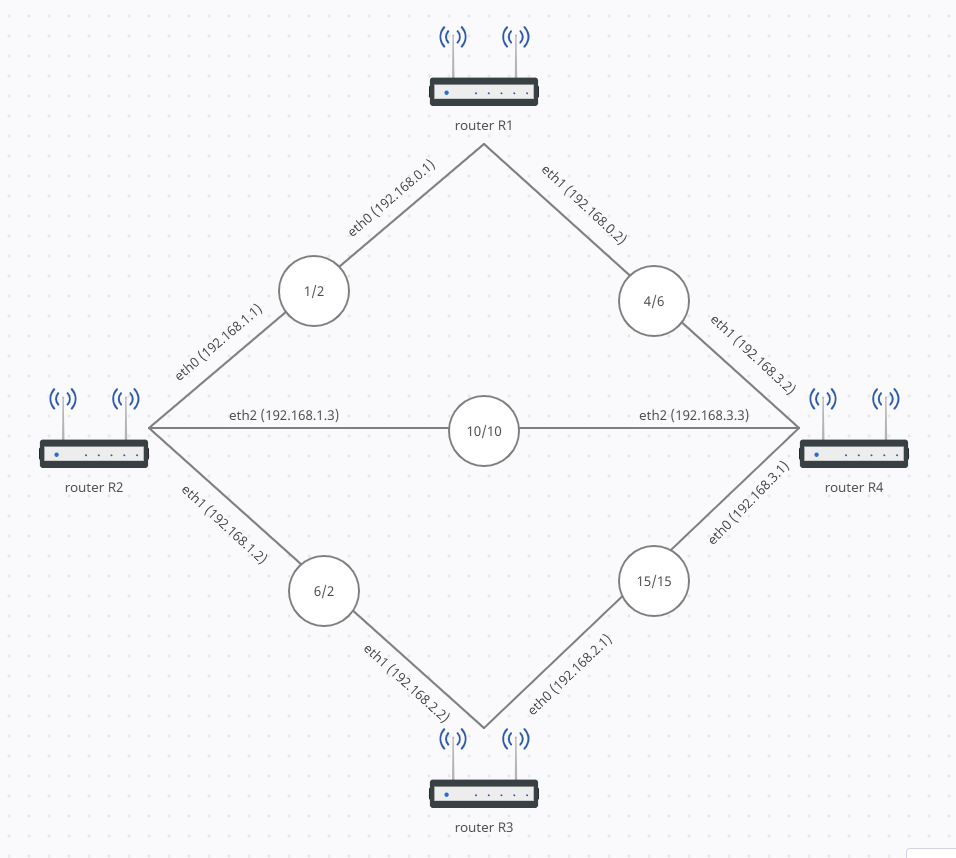
\includegraphics[width=0.65\textwidth]{../documents/topology-figure.png}
  \caption{Topologie de 4 nœuds et 5 liens}
   \label{fig:topology}
\end{figure}
\begin{figure} [h!]
\centering
  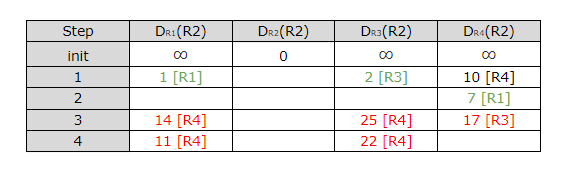
\includegraphics[width=0.65\textwidth]{../documents/demo-table.png}
  \caption{Tableau des routes calculées par les routeurs vers R2}
   \label{fig:table}
\end{figure}
La Figure \ref{fig:topology} représente une topologie contenant 4 nœuds et 5 liens ainsi que les coûts et les interfaces par lesquelles ils sont connectés. La figure \ref{fig:table} quant à elle, représente les routes calculées à partir de chacun des routeurs vers une unique destination \textit{(R2)}.

\section{Exercice 2.3}
\begin{figure} [h!]
\centering
  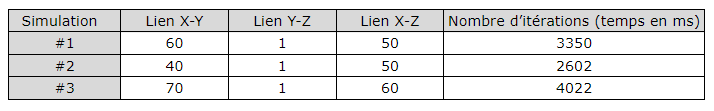
\includegraphics[width=0.65\textwidth]{../documents/infinity-table.png}
  \caption{Tableau contenant 3 simulations différentes}
   \label{fig:inf-table}
\end{figure}
\textit{Votre rapport doit contenir la topologie mise en oeuvre pour reproduire le comptage à l’infini en cas de changement de métrique}.\\

\textit{Il doit également indiquer le nombre de messages échangés par les routeurs (i.e. nombre d’itérations) depuis le changement de métrique et jusqu’à la nouvelle convergence.}\\

Les 2 assignements de coûts de liens qui résultent en une convergence plus courte et une autre plus longue sont renseignés dans la Figure \ref{fig:inf-table}.

\section{Exercice 2.4}
La nom de la solution au comptage à l'infini vue dans le cours est \textit{Poisoned reverse}. Elle consiste à ne pas indiquer le coût réel vers la destination aux voisins (en leur envoyant $+\infty$ comme coût) qui passent par ce même nœud afin d'éviter le problème de comptage à l'infini. Dans la topologie donnée dans l'exercice 2.3, Y doit renseigner $+\infty$ à Z --- son voisin --- puisque celui-ci passe pas Y afin d'atteindre X ; sa destination.\\

\textit{Décrivez dans le rapport, en maximum 5 lignes, pourquoi le problème persiste dans ce cas
exceptionnel}\\

\textit{Proposez dans le rapport un mécanisme qui permettrait de résoudre ce nouveau
problème}

\section{Evaluation via génération de topologies}
\textit{Le rapport doit contenir un graphique (ou un tableau) contenant les temps de convergence obtenus
pour chaque nombre de liens.}

\vspace{10px}
\begin{center}
\end{center}

\topskip0pt
\vspace*{\fill}

\end{document}